% Options for packages loaded elsewhere
\PassOptionsToPackage{unicode}{hyperref}
\PassOptionsToPackage{hyphens}{url}
%
\documentclass[
]{article}
\usepackage{amsmath,amssymb}
\usepackage{lmodern}
\usepackage{ifxetex,ifluatex}
\ifnum 0\ifxetex 1\fi\ifluatex 1\fi=0 % if pdftex
  \usepackage[T1]{fontenc}
  \usepackage[utf8]{inputenc}
  \usepackage{textcomp} % provide euro and other symbols
\else % if luatex or xetex
  \usepackage{unicode-math}
  \defaultfontfeatures{Scale=MatchLowercase}
  \defaultfontfeatures[\rmfamily]{Ligatures=TeX,Scale=1}
\fi
% Use upquote if available, for straight quotes in verbatim environments
\IfFileExists{upquote.sty}{\usepackage{upquote}}{}
\IfFileExists{microtype.sty}{% use microtype if available
  \usepackage[]{microtype}
  \UseMicrotypeSet[protrusion]{basicmath} % disable protrusion for tt fonts
}{}
\makeatletter
\@ifundefined{KOMAClassName}{% if non-KOMA class
  \IfFileExists{parskip.sty}{%
    \usepackage{parskip}
  }{% else
    \setlength{\parindent}{0pt}
    \setlength{\parskip}{6pt plus 2pt minus 1pt}}
}{% if KOMA class
  \KOMAoptions{parskip=half}}
\makeatother
\usepackage{xcolor}
\IfFileExists{xurl.sty}{\usepackage{xurl}}{} % add URL line breaks if available
\IfFileExists{bookmark.sty}{\usepackage{bookmark}}{\usepackage{hyperref}}
\hypersetup{
  pdftitle={Data wrangling},
  hidelinks,
  pdfcreator={LaTeX via pandoc}}
\urlstyle{same} % disable monospaced font for URLs
\usepackage[margin=1in]{geometry}
\usepackage{color}
\usepackage{fancyvrb}
\newcommand{\VerbBar}{|}
\newcommand{\VERB}{\Verb[commandchars=\\\{\}]}
\DefineVerbatimEnvironment{Highlighting}{Verbatim}{commandchars=\\\{\}}
% Add ',fontsize=\small' for more characters per line
\usepackage{framed}
\definecolor{shadecolor}{RGB}{248,248,248}
\newenvironment{Shaded}{\begin{snugshade}}{\end{snugshade}}
\newcommand{\AlertTok}[1]{\textcolor[rgb]{0.94,0.16,0.16}{#1}}
\newcommand{\AnnotationTok}[1]{\textcolor[rgb]{0.56,0.35,0.01}{\textbf{\textit{#1}}}}
\newcommand{\AttributeTok}[1]{\textcolor[rgb]{0.77,0.63,0.00}{#1}}
\newcommand{\BaseNTok}[1]{\textcolor[rgb]{0.00,0.00,0.81}{#1}}
\newcommand{\BuiltInTok}[1]{#1}
\newcommand{\CharTok}[1]{\textcolor[rgb]{0.31,0.60,0.02}{#1}}
\newcommand{\CommentTok}[1]{\textcolor[rgb]{0.56,0.35,0.01}{\textit{#1}}}
\newcommand{\CommentVarTok}[1]{\textcolor[rgb]{0.56,0.35,0.01}{\textbf{\textit{#1}}}}
\newcommand{\ConstantTok}[1]{\textcolor[rgb]{0.00,0.00,0.00}{#1}}
\newcommand{\ControlFlowTok}[1]{\textcolor[rgb]{0.13,0.29,0.53}{\textbf{#1}}}
\newcommand{\DataTypeTok}[1]{\textcolor[rgb]{0.13,0.29,0.53}{#1}}
\newcommand{\DecValTok}[1]{\textcolor[rgb]{0.00,0.00,0.81}{#1}}
\newcommand{\DocumentationTok}[1]{\textcolor[rgb]{0.56,0.35,0.01}{\textbf{\textit{#1}}}}
\newcommand{\ErrorTok}[1]{\textcolor[rgb]{0.64,0.00,0.00}{\textbf{#1}}}
\newcommand{\ExtensionTok}[1]{#1}
\newcommand{\FloatTok}[1]{\textcolor[rgb]{0.00,0.00,0.81}{#1}}
\newcommand{\FunctionTok}[1]{\textcolor[rgb]{0.00,0.00,0.00}{#1}}
\newcommand{\ImportTok}[1]{#1}
\newcommand{\InformationTok}[1]{\textcolor[rgb]{0.56,0.35,0.01}{\textbf{\textit{#1}}}}
\newcommand{\KeywordTok}[1]{\textcolor[rgb]{0.13,0.29,0.53}{\textbf{#1}}}
\newcommand{\NormalTok}[1]{#1}
\newcommand{\OperatorTok}[1]{\textcolor[rgb]{0.81,0.36,0.00}{\textbf{#1}}}
\newcommand{\OtherTok}[1]{\textcolor[rgb]{0.56,0.35,0.01}{#1}}
\newcommand{\PreprocessorTok}[1]{\textcolor[rgb]{0.56,0.35,0.01}{\textit{#1}}}
\newcommand{\RegionMarkerTok}[1]{#1}
\newcommand{\SpecialCharTok}[1]{\textcolor[rgb]{0.00,0.00,0.00}{#1}}
\newcommand{\SpecialStringTok}[1]{\textcolor[rgb]{0.31,0.60,0.02}{#1}}
\newcommand{\StringTok}[1]{\textcolor[rgb]{0.31,0.60,0.02}{#1}}
\newcommand{\VariableTok}[1]{\textcolor[rgb]{0.00,0.00,0.00}{#1}}
\newcommand{\VerbatimStringTok}[1]{\textcolor[rgb]{0.31,0.60,0.02}{#1}}
\newcommand{\WarningTok}[1]{\textcolor[rgb]{0.56,0.35,0.01}{\textbf{\textit{#1}}}}
\usepackage{graphicx}
\makeatletter
\def\maxwidth{\ifdim\Gin@nat@width>\linewidth\linewidth\else\Gin@nat@width\fi}
\def\maxheight{\ifdim\Gin@nat@height>\textheight\textheight\else\Gin@nat@height\fi}
\makeatother
% Scale images if necessary, so that they will not overflow the page
% margins by default, and it is still possible to overwrite the defaults
% using explicit options in \includegraphics[width, height, ...]{}
\setkeys{Gin}{width=\maxwidth,height=\maxheight,keepaspectratio}
% Set default figure placement to htbp
\makeatletter
\def\fps@figure{htbp}
\makeatother
\setlength{\emergencystretch}{3em} % prevent overfull lines
\providecommand{\tightlist}{%
  \setlength{\itemsep}{0pt}\setlength{\parskip}{0pt}}
\setcounter{secnumdepth}{-\maxdimen} % remove section numbering
\usepackage{booktabs}
\usepackage{longtable}
\usepackage{array}
\usepackage{multirow}
\usepackage{wrapfig}
\usepackage{float}
\usepackage{colortbl}
\usepackage{pdflscape}
\usepackage{tabu}
\usepackage{threeparttable}
\usepackage{threeparttablex}
\usepackage[normalem]{ulem}
\usepackage{makecell}
\usepackage{xcolor}
\ifluatex
  \usepackage{selnolig}  % disable illegal ligatures
\fi

\title{Data wrangling}
\author{}
\date{\vspace{-2.5em}}

\begin{document}
\maketitle

\hypertarget{raw}{%
\section{Raw}\label{raw}}

\hypertarget{read-text}{%
\section{Read text}\label{read-text}}

\begin{Shaded}
\begin{Highlighting}[]
\NormalTok{read\_story }\OtherTok{\textless{}{-}} \ControlFlowTok{function}\NormalTok{(x) \{}
\NormalTok{  text }\OtherTok{\textless{}{-}} \FunctionTok{read\_html}\NormalTok{(x) }\SpecialCharTok{\%\textgreater{}\%} 
  \FunctionTok{html\_nodes}\NormalTok{(}\StringTok{"p"}\NormalTok{) }\SpecialCharTok{\%\textgreater{}\%} 
  \FunctionTok{html\_text}\NormalTok{() }\SpecialCharTok{\%\textgreater{}\%} 
\NormalTok{  glue}\SpecialCharTok{::}\FunctionTok{glue\_collapse}\NormalTok{(}\AttributeTok{sep =} \StringTok{" "}\NormalTok{)}
  
  \FunctionTok{return}\NormalTok{(text)}
\NormalTok{\}}

\NormalTok{story\_text\_list }\OtherTok{\textless{}{-}}\NormalTok{ detective\_data }\SpecialCharTok{\%\textgreater{}\%} 
  \FunctionTok{filter}\NormalTok{(}\SpecialCharTok{!}\FunctionTok{str\_detect}\NormalTok{(story\_url, }\StringTok{".txt"}\NormalTok{)) }\SpecialCharTok{\%\textgreater{}\%} 
  \FunctionTok{filter}\NormalTok{(}\SpecialCharTok{!}\FunctionTok{str\_detect}\NormalTok{(story\_url, }\StringTok{" "}\NormalTok{)) }\SpecialCharTok{\%\textgreater{}\%} 
  \FunctionTok{filter}\NormalTok{(}\SpecialCharTok{!}\FunctionTok{str\_detect}\NormalTok{(story\_url, }\StringTok{"\#"}\NormalTok{)) }\SpecialCharTok{\%\textgreater{}\%} 
  \FunctionTok{select}\NormalTok{(story\_url, story\_code, what\_is\_the\_reveal\_border\_sentence)}

\CommentTok{\# Take a while to run}
\CommentTok{\# story\_text \textless{}{-} map\_dfr(.x = c(url = story\_text\_list$story\_url), .f = read\_story)}

\CommentTok{\# saveRDS(story\_text, "story\_text.rds")}
\end{Highlighting}
\end{Shaded}

\begin{Shaded}
\begin{Highlighting}[]
\NormalTok{story\_text }\OtherTok{\textless{}{-}} \FunctionTok{readRDS}\NormalTok{(}\StringTok{"story\_text.rds"}\NormalTok{)}

\NormalTok{story\_text\_list }\OtherTok{\textless{}{-}}\NormalTok{ detective\_data }\SpecialCharTok{\%\textgreater{}\%} 
  \FunctionTok{filter}\NormalTok{(}\SpecialCharTok{!}\FunctionTok{str\_detect}\NormalTok{(story\_url, }\StringTok{".txt"}\NormalTok{)) }\SpecialCharTok{\%\textgreater{}\%} 
  \FunctionTok{filter}\NormalTok{(}\SpecialCharTok{!}\FunctionTok{str\_detect}\NormalTok{(story\_url, }\StringTok{" "}\NormalTok{)) }\SpecialCharTok{\%\textgreater{}\%} 
  \FunctionTok{filter}\NormalTok{(}\SpecialCharTok{!}\FunctionTok{str\_detect}\NormalTok{(story\_url, }\StringTok{"\#"}\NormalTok{)) }\SpecialCharTok{\%\textgreater{}\%} 
  \FunctionTok{select}\NormalTok{(story\_url, story\_code, what\_is\_the\_reveal\_border\_sentence)}

\NormalTok{story\_text\_clean }\OtherTok{\textless{}{-}}\NormalTok{ story\_text }\SpecialCharTok{\%\textgreater{}\%} 
  \FunctionTok{pivot\_longer}\NormalTok{(}\FunctionTok{everything}\NormalTok{(), }\AttributeTok{values\_to =} \StringTok{"text"}\NormalTok{) }\SpecialCharTok{\%\textgreater{}\%} 
  \FunctionTok{select}\NormalTok{(}\SpecialCharTok{{-}}\NormalTok{name) }\SpecialCharTok{\%\textgreater{}\%} 
  \FunctionTok{mutate}\NormalTok{(}\AttributeTok{story\_code =}\NormalTok{ story\_text\_list}\SpecialCharTok{$}\NormalTok{story\_code, }
         \AttributeTok{what\_is\_the\_reveal\_border\_sentence =}\NormalTok{ story\_text\_list}\SpecialCharTok{$}\NormalTok{what\_is\_the\_reveal\_border\_sentence) }\SpecialCharTok{\%\textgreater{}\%} 
  \FunctionTok{mutate}\NormalTok{(}\AttributeTok{text\_length =} \FunctionTok{str\_count}\NormalTok{(text)}\SpecialCharTok{+}\DecValTok{1}\NormalTok{)}

\FunctionTok{head}\NormalTok{(story\_text\_clean)}
\end{Highlighting}
\end{Shaded}

\begin{verbatim}
## # A tibble: 6 x 4
##   text                    story_code what_is_the_reveal_border_sent~ text_length
##   <glue>                  <chr>      <chr>                                 <dbl>
## 1 "\n“I am afraid, Watso~ MSH01      "Sherlock Holmes laughed. “I a~       52248
## 2 "[In publishing these ~ MSH02      "“I will tell you the meaning ~       39240
## 3 "\nShortly after my ma~ MSH03      "“Oh surely if you consider th~       34298
## 4 "\nThe Lord St. Simon ~ ASH10      "“The best possible.”"                39198
## 5 "\n“Holmes,” said I as~ ASH11      "\"For heaven's sake, tell me,~       50716
## 6 "\n“To the man who lov~ ASH12      "If there's police-court busin~       51513
\end{verbatim}

\begin{Shaded}
\begin{Highlighting}[]
\NormalTok{only\_reveals }\OtherTok{\textless{}{-}}\NormalTok{ story\_text\_clean }\SpecialCharTok{\%\textgreater{}\%} 
  \FunctionTok{select}\NormalTok{(what\_is\_the\_reveal\_border\_sentence) }\SpecialCharTok{\%\textgreater{}\%} 
  \FunctionTok{filter}\NormalTok{(}\SpecialCharTok{!}\FunctionTok{is.na}\NormalTok{(what\_is\_the\_reveal\_border\_sentence))}

\NormalTok{my\_sep }\OtherTok{\textless{}{-}}\NormalTok{ glue}\SpecialCharTok{::}\FunctionTok{glue\_collapse}\NormalTok{(only\_reveals}\SpecialCharTok{$}\NormalTok{what\_is\_the\_reveal\_border\_sentence, }\AttributeTok{sep =} \StringTok{"|"}\NormalTok{)}

\NormalTok{split }\OtherTok{\textless{}{-}}\NormalTok{ story\_text\_clean }\SpecialCharTok{\%\textgreater{}\%} 
  \FunctionTok{mutate}\NormalTok{(}\AttributeTok{text\_words =} \FunctionTok{str\_count}\NormalTok{(text)}\SpecialCharTok{+}\DecValTok{1}\NormalTok{) }\SpecialCharTok{\%\textgreater{}\%} 
  \FunctionTok{rowwise}\NormalTok{() }\SpecialCharTok{\%\textgreater{}\%} 
  \FunctionTok{separate}\NormalTok{(text, }\AttributeTok{into =} \FunctionTok{c}\NormalTok{(}\StringTok{"before\_reveal"}\NormalTok{, }\StringTok{"after\_reveal"}\NormalTok{, }\StringTok{"uhoh"}\NormalTok{), }\AttributeTok{sep =}\NormalTok{ my\_sep) }\SpecialCharTok{\%\textgreater{}\%} 
  \FunctionTok{mutate}\NormalTok{(}\AttributeTok{after\_reveal =} \FunctionTok{if\_else}\NormalTok{(}\FunctionTok{is.na}\NormalTok{(uhoh), after\_reveal, uhoh)) }\SpecialCharTok{\%\textgreater{}\%} 
  \FunctionTok{select}\NormalTok{(}\SpecialCharTok{{-}}\NormalTok{uhoh) }\SpecialCharTok{\%\textgreater{}\%} 
  \FunctionTok{mutate}\NormalTok{(}\AttributeTok{before\_reveal\_words =} \FunctionTok{str\_count}\NormalTok{(before\_reveal)}\SpecialCharTok{+}\DecValTok{1}\NormalTok{,}
         \AttributeTok{after\_reveal\_words =} \FunctionTok{str\_count}\NormalTok{(after\_reveal)}\SpecialCharTok{+}\DecValTok{1}\NormalTok{)}
\end{Highlighting}
\end{Shaded}

\begin{verbatim}
## Warning: Expected 3 pieces. Missing pieces filled with `NA` in 126 rows [1, 2,
## 3, 4, 5, 6, 7, 8, 9, 10, 11, 12, 13, 14, 15, 16, 17, 18, 19, 20, ...].
\end{verbatim}

\begin{Shaded}
\begin{Highlighting}[]
\NormalTok{split }\SpecialCharTok{\%\textgreater{}\%} 
  \FunctionTok{ggplot}\NormalTok{(}\FunctionTok{aes}\NormalTok{(}\AttributeTok{x =}\NormalTok{ text\_words, }\AttributeTok{y =}\NormalTok{ after\_reveal\_words)) }\SpecialCharTok{+}
  \FunctionTok{geom\_point}\NormalTok{()}
\end{Highlighting}
\end{Shaded}

\begin{verbatim}
## Warning: Removed 29 rows containing missing values (geom_point).
\end{verbatim}

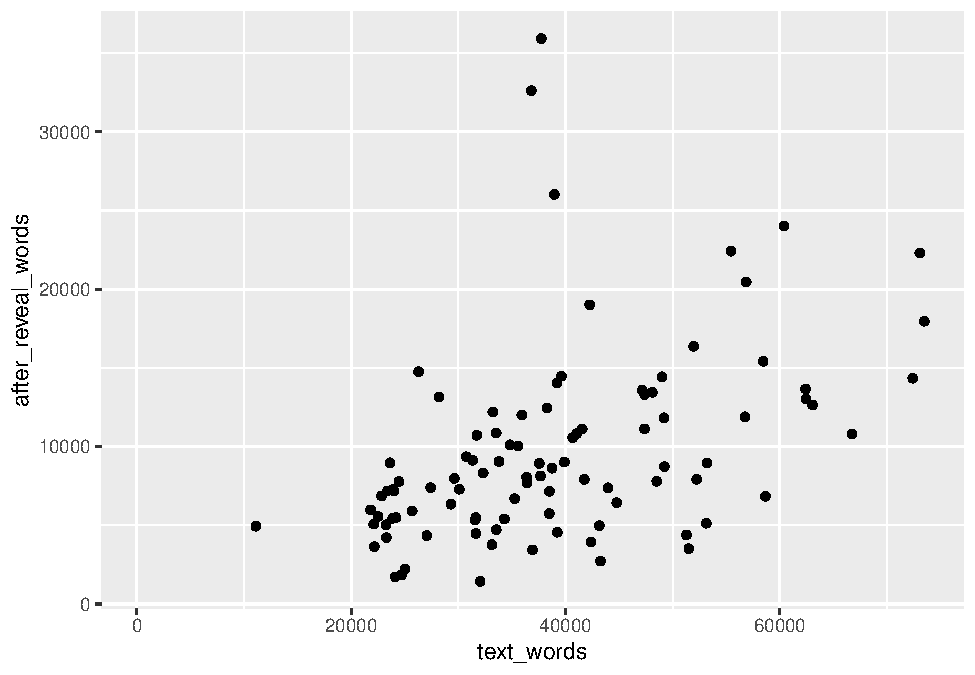
\includegraphics{data-wrangling_files/figure-latex/unnamed-chunk-6-1.pdf}

\begin{Shaded}
\begin{Highlighting}[]
\NormalTok{word\_counts\_text }\OtherTok{\textless{}{-}}\NormalTok{ split }\SpecialCharTok{\%\textgreater{}\%} 
  \FunctionTok{select}\NormalTok{(story\_code, }\FunctionTok{contains}\NormalTok{(words))}
\end{Highlighting}
\end{Shaded}

\begin{Shaded}
\begin{Highlighting}[]
\NormalTok{detective\_data\_1 }\OtherTok{\textless{}{-}}\NormalTok{ detective\_data }\SpecialCharTok{\%\textgreater{}\%} 
  \FunctionTok{left\_join}\NormalTok{(word\_counts\_text, }\AttributeTok{by =} \StringTok{"story\_code"}\NormalTok{) }\SpecialCharTok{\%\textgreater{}\%} 
  \FunctionTok{mutate}\NormalTok{(}\AttributeTok{title\_words =} \FunctionTok{str\_count}\NormalTok{(story\_name)}\SpecialCharTok{+}\DecValTok{1}\NormalTok{) }\SpecialCharTok{\%\textgreater{}\%} 
  \FunctionTok{mutate}\NormalTok{(}\AttributeTok{before\_reveal\_words =} \FunctionTok{if\_else}\NormalTok{(}\FunctionTok{is.na}\NormalTok{(after\_reveal\_words), }\ConstantTok{NaN}\NormalTok{, before\_reveal\_words))}
\end{Highlighting}
\end{Shaded}

\begin{Shaded}
\begin{Highlighting}[]
\NormalTok{my\_skim }\OtherTok{\textless{}{-}} \FunctionTok{skim}\NormalTok{(detective\_data)}
\NormalTok{data\_dic }\OtherTok{\textless{}{-}} \FunctionTok{tibble}\NormalTok{(}\AttributeTok{variable\_name =}\NormalTok{ my\_skim}\SpecialCharTok{$}\NormalTok{skim\_variable,}
                   \AttributeTok{data\_type =}\NormalTok{ my\_skim}\SpecialCharTok{$}\NormalTok{skim\_type)}

\NormalTok{knitr}\SpecialCharTok{::}\FunctionTok{kable}\NormalTok{(data\_dic) }\SpecialCharTok{\%\textgreater{}\%} 
\NormalTok{  kableExtra}\SpecialCharTok{::}\FunctionTok{column\_spec}\NormalTok{(}\DecValTok{1}\NormalTok{, }\AttributeTok{width =} \StringTok{"10em"}\NormalTok{) }\SpecialCharTok{\%\textgreater{}\%} 
\NormalTok{  kableExtra}\SpecialCharTok{::}\FunctionTok{kable\_styling}\NormalTok{(}\AttributeTok{full\_width =} \ConstantTok{TRUE}\NormalTok{)}
\end{Highlighting}
\end{Shaded}

\begin{tabu} to \linewidth {>{\raggedright\arraybackslash}p{10em}>{\raggedright}X}{>{\raggedright\arraybackslash}p{10em}|l}
\hline
variable\_name & data\_type\\
\hline
story\_code & character\\
\hline
story\_name & character\\
\hline
plot\_summary\_25\_50\_words & character\\
\hline
author\_code & character\\
\hline
in\_what\_order\_are\_the\_investigation\_and\_reveal\_portions\_provided & character\\
\hline
name\_of\_detective\_number\_1 & character\\
\hline
detective\_number\_1\_gender & character\\
\hline
detective\_number\_1\_role & character\\
\hline
name\_of\_detective\_number\_2 & character\\
\hline
detective\_number\_2\_gender & character\\
\hline
detective\_number\_2\_role & character\\
\hline
name\_of\_assistant\_number\_1 & character\\
\hline
assistant\_number\_1\_gender & character\\
\hline
assistant\_number\_1\_role & character\\
\hline
name\_of\_assistant\_number\_2 & character\\
\hline
assistant\_number\_2\_gender & character\\
\hline
assistant\_number\_2\_role & character\\
\hline
are\_one\_or\_more\_culprits\_introduced\_into\_the\_story\_only\_during\_the\_reveal & character\\
\hline
the\_main\_culprit & character\\
\hline
who\_initiates\_the\_detectives\_investigation & character\\
\hline
what\_is\_the\_role\_of\_the\_police\_force\_in\_solving\_the\_crime & character\\
\hline
the\_storys\_main\_action\_focuses\_on\_a & character\\
\hline
when\_do\_es\_the\_crime\_s\_mystery\_being\_investigated\_occur & character\\
\hline
types\_of\_crimes\_or\_quasi\_crimes\_present\_in\_story & character\\
\hline
motives & character\\
\hline
means\_murder\_only & character\\
\hline
does\_the\_story\_provide\_sufficient\_clues\_in\_sufficient\_detail\_to\_allow\_an\_alert\_reader\_to\_correctly\_guess\_the\_solution\_before\_the\_reveal & character\\
\hline
does\_the\_story\_provide\_sufficient\_clues\_in\_sufficient\_detail\_to\_allow\_an\_alert\_reader\_to\_definitively\_solve\_the\_crime\_before\_the\_reveal & character\\
\hline
did\_either\_annotator\_personally\_correctly\_guess\_the\_solution\_to\_the\_crime\_before\_the\_reveal & character\\
\hline
types\_of\_clues & character\\
\hline
what\_is\_the\_essential\_clue\_in\_the\_story\_if\_present & character\\
\hline
of\_what\_type\_is\_the\_essential\_clue\_if\_present & character\\
\hline
what\_is\_the\_most\_salient\_clue\_in\_the\_story\_if\_clues\_are\_present & character\\
\hline
of\_what\_type\_is\_the\_most\_salient\_clue\_if\_clues\_are\_present & character\\
\hline
describe\_the\_main\_red\_herring\_if\_present & character\\
\hline
of\_what\_type\_is\_the\_main\_red\_herring\_if\_present & character\\
\hline
presence\_of\_planted\_or\_fabricated\_evidence & character\\
\hline
types\_of\_evidence\_made\_available\_in\_the\_story & character\\
\hline
is\_the\_crime\_solved & character\\
\hline
does\_the\_detective\_pointedly\_and\_independently\_decide\_not\_to\_alert\_the\_authorities\_to\_the\_facts\_of\_the\_crime\_despite\_the\_fact\_that\_an\_actionable\_crime\_has\_been\_committed & character\\
\hline
do\_you\_receive\_a\_satisfying\_narrative\_of\_account\_of\_the\_crime\_s\_in\_all\_their\_relevant\_details\_and\_a\_summary\_of\_the\_process\_by\_which\_the\_crime\_s\_are\_solved & character\\
\hline
would\_you\_recommend\_this\_story\_to\_a\_friend & character\\
\hline
crime\_trajectory & character\\
\hline
what\_is\_the\_reveal\_border\_sentence & character\\
\hline
surname\_s & character\\
\hline
given\_name\_s & character\\
\hline
sex & character\\
\hline
country\_of\_birth & character\\
\hline
city\_town\_of\_birth & character\\
\hline
country\_of\_death & character\\
\hline
city\_town\_of\_death & character\\
\hline
nationality\_ies & character\\
\hline
viaf & character\\
\hline
story\_url & character\\
\hline
format\_of\_first\_publication\_journal\_or\_book & character\\
\hline
name\_of\_journal\_or\_title\_of\_book & character\\
\hline
second\_author\_code\_if\_applicable & logical\\
\hline
more\_than\_two\_detectives\_if\_yes\_enter\_total\_number & logical\\
\hline
number\_of\_victims\_of\_gender\_non\_binary & logical\\
\hline
number\_of\_victims\_of\_gender\_unknown & logical\\
\hline
number\_of\_victims\_who\_are\_corporate\_entities & logical\\
\hline
more\_than\_two\_assistants\_if\_yes\_enter\_total\_number & numeric\\
\hline
number\_of\_victims\_of\_gender\_male & numeric\\
\hline
number\_of\_victims\_of\_gender\_female & numeric\\
\hline
number\_of\_culprits\_of\_gender\_male & numeric\\
\hline
number\_of\_culprits\_of\_gender\_female & numeric\\
\hline
number\_of\_culprits\_of\_gender\_non\_binary & numeric\\
\hline
number\_of\_culprits\_of\_gender\_unknown & numeric\\
\hline
how\_satisfying\_is\_this\_story\_as\_a\_piece\_of\_detective\_fiction & numeric\\
\hline
year\_of\_birth & POSIXct\\
\hline
date\_of\_death\_yyyy\_mm\_dd & POSIXct\\
\hline
date\_of\_first\_publication\_yyyy\_mm\_dd & POSIXct\\
\hline
\end{tabu}

\end{document}
